\documentclass[twopage,11pt]{article}

% Any additional packages needed should be included after jmlr2e.
% Note that jmlr2e.sty includes epsfig, amssymb, natbib and graphicx,
% and defines many common macros, such as 'proof' and 'example'.
%
% It also sets the bibliographystyle to plainnat; for more information on
% natbib citation styles, see the natbib documentation, a copy of which
% is archived at http://www.jmlr.org/format/natbib.pdf

\usepackage{jmlr2e}
\usepackage{graphicx}% Definitions of handy macros can go here
\usepackage{hyperref}

\newcommand{\dataset}{{\cal D}}
\newcommand{\fracpartial}[2]{\frac{\partial #1}{\partial  #2}}

% Heading arguments are {volume}{year}{pages}{submitted}{published}{author-full-names}

\jmlrheading{1}{2008}{1-48}{4/00}{10/00}{RL-Glue Tanner and White}

% Short headings should be running head and authors last names

\ShortHeadings{RL-Glue}{Tanner and White}
\firstpageno{1}

\begin{document}

\title{The RL-Glue Software Project: An Open Source Framework for Reinforcement Learning Experiments}

\author{\name Brian Tanner \AND Adam White  \email \{btanner,awhite\}@cs.ualberta.ca \\
       \addr Department of Computing Science\\
       University of Alberta\\
       Edmonton, AB 98195-4322, Canada}

\editor{ Soeren Sonnenburg}

\maketitle

\begin{abstract}
%Note: will fix this later. still represents the paper well. but needs to be touched up
RL-Glue is a open source system for implementing and evaluating reinforcement learning experiments. Standardization can facilitate efficient code sharing and collaboration removing the need to re-implement code to reproduce and verify others results.  RL-Glue is well suited for empirical research, course work and industrial scale projects. Our software features a minimal interface and supports C, C++, Java, Python, Matlab and Lisp and runs on Linux, Macintosh, and Windows natively. RL-Glue can be easily extended to support additional programing languages and other evaluation software using a TCP/IP interface. RL-Glue has been used to evaluate performance in several international competitions and is currently used by several other open-source software and hardware projects.
\end{abstract}

\section{Introduction and Motivation}
In reinforcement learning an {\it agent} learns the effects of its {\it actions} through trail and error interaction with the {\it environment} \cite{rlbook, rlsurvey,ndp}. The agent selects actions based on its {\it observation} of the state of the environment and a scalar {\it reward} signal. The agent's objective is to select actions which maximize the sum of future rewards. The observations and rewards produced by the environment are conditioned on the actions taken by the agent; the environment cannot be encoded in a data-file like in supervised learning. In reinforcement learning the agent and environment must be interacting programs. 

 


The many reinforcement learning researchers use different interfaces and packages to test learning algorithms: this makes collaboration difficult and can also limit the growth of the community. It is can be difficult and time consuming to re-implement other's code, especially when environment details and agent optimizations are not specified. Several well-known environments are publicly available in several variations, all refereed to as the "standard" implementation \cite{whiteThesis}. There has also been significant interest, in recent years, in establishing annual agent competitions and benchmark problems, necessitating a standard evaluation system for reinforcement learning. The RL-Glue Software Project is meant alleviate the evaluation difficulties facing reinforcement learning practitioners.


















 



	 

\section{RL-Glue}

\begin{figure}[h]
\begin{center}
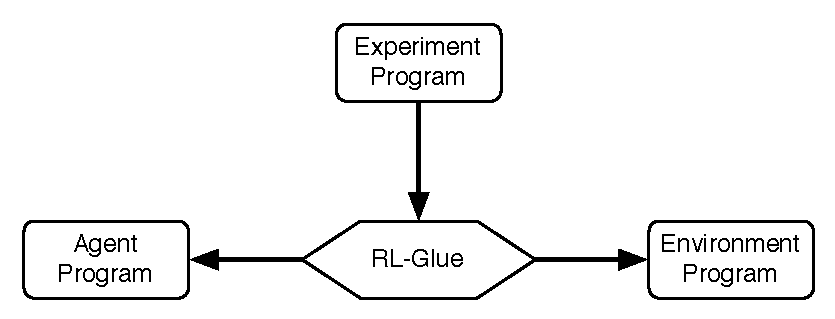
\includegraphics[width = 9 cm]{glue.pdf}
\vspace{-0.2cm}
\caption{\small The RL-Glue system architecture. Arrows indicate function call direction.}\label{fig:RLDIA}
\end{center}
\vspace{-0.4cm}
\end{figure}

The RL-Glue Software is an implementation of the RL-Glue protocol \cite{whitesutton}. The RL-Glue protocol is a standard for communication between agent and environment programs. The RL-Glue protocol separates the the reinforcement learning framework into four main components: the agent, environment, experiment program and the RL-Glue interface. The agent contains the learning algorithm and action selection mechanism. The environment is the problem. The experiment program specifies the remaining details concerning the experiment execution including the number and sequence of interactions, data collection and processing.  The RL-Glue components is a simple interface that calls agent and environment functions in response to function calls from the experiment program (See Figure \ref{fig:RLDIA}). 

The RL-Glue software is a language independent implemention of the RL-Glue protocol  that allows agent, environment and experiment programs to be developed in different languages, and run on different computers over the internet. 

RL-Glue can be run in {\it native} or {\it network} mode to maximize plug and play and personalize the system. In native mode, the agent, environment and experiment program are compiled into a single C, C++ executable. In networked mode, the agent, environment and experiment program communicate with RL-Glue over a TCP/IP socket connection. The native mode's primary strength is speed of execution, while the network mode allows cross language communication and interfacing with other software projects. The agent or environment program are completely agnostic of the execution mode.       

The network mode allows the agent, environment and experiment programs to be written in any programing language. In fact, any language that supports socket I/O can be made compatible with RL-Glue. The current release of the RL-Glue Software includes support for Java, C/C++, Matlab, Python and Lisp.  
\\\\
{\bf Task Spec ....}



\section{$<$RL-Glue Related Projects$>$}
RL-Glue has had a significant impact on the reinforcement learning community and has been used in several projects. The reinforcement learning library\footnote{http://library.rl-community.org/} (RL-Libary) is mechanism for sharing RL-Glue compatible code. RL-Library is a public repository of agent, environment, experiment and utility programs for the reinforcement learning community. The RL-Library is an open-source project that promotes submissions of RL-Glue related codes. RL-Viz\footnote{http://code.google.com/p/rl-viz/} is an API layered on top of RL-Glue. RL-Viz can be used to dynamically load agent and environment programs, modify parameters at runtime and visualize interaction and performance.  The reinforcement learning competition\footnote{http://www.rl-competition.org/} is an annual event where teams from around the world compare their learning algorithms on a variety of challenging environments. RL-Glue has been used as the evaluation system for all three events. Finally, the Critter Bot\footnote{http://www.cs.ualberta.ca/$\sim$sokolsky/critterbot/} is an mobile robot that is outfitted with a unusually rich set of subjective sensors. The robot is compatible with rl-glue; agents developed for simulated environments can easily employed on the robot.

The socket architecture of RL-Glue can be used to connect agent programs to other software projects. Currently socket bridges exist for connecting RL-Glue to a keepaway soccer server, a real-time strategy game engine and an Atari emulator. Our socket architecture helps lower the barriers for researchers wishing to work on larger scale environments by providing with a simple and familiar interface. These environments will soon be accessible via RL-Library. 


RL-Glue has been used for teaching reinforcement learning in several university courses and evaluating learning performance in papers published in leading conferences. An up-to-date list of what RL-Glue is used for can be found online at: {\url http://glue.rl-community.org/rl-glue-in-practice}




\section{Other Reinforcement Learning Software Projects}

There are several other software projects that introduce an interface for reinforcement learning experiments. CL$^2$ provides much of the functionality of RL-Glue, but only supports C++ and uses parameter files to specify the experiment program. PIQLE is a Java system that provides some of the functionality of RL-Glue and supports multi-agent reinforcement learning. PIQLE, however, does not provide important experimental control or continuous action types. RL Toolbox is an object oriented C++ package that is distributed with many built-in learning algorithms. Other, less popular, reinforcement learning packages include JRLF and libpg. 

Some of these alternative packages are distributed with a number agents and environments which are of interest to RL-Glue users. RL-Glue has been designed to minimize the barriers to converting existing programs to run under RL-Glue. Additionally, we are currently making RLToolbox algorithms and problems compatible with RL-Glue. 






 
 
 
\section{RL-Glue Open Source Project}
%NOTE: I am thinking about removing codecs from the paper ...

RL-Glue is not just an evaluation tool or development environment: RL-Glue is a community project with many levels of possible participation. The easiest and most obvious way to participate is to submit agent, environment and experiment programs to RL-Library. Developers can also help extend RL-Glue compatibility to additional languages by submitting new codecs. The RL-Glue project welcomes code submissions and improvements for all parts of the code base.   	

The RL-Glue Software Project has received significant contributions at many of the levels discussed above. The Lisp codecs were contributed by Gabor Balazs. Jose Antonio Martin H. developed a native windows implementation of RL-Glue. Quickly list library contributions ....

RL-Glue is available under the Apache License, Version 2.0.
	

\section{History of RL-Glue}
RL-Glue 1.0\\
2.0\\
3.0
\\\\
Give credit at each stage

\addcontentsline{toc}{chapter}{Bibliography}
     %add the above line to get "Bibliography" in the table of contents.
%
%\singlespacing % optional;  Bibliography is better in single spacing
               %            but you may choose different
               %            Don't use \singlespacing if your thesis
               %            is already in single spacing
%
\bibliographystyle{plain} % Or which ever you wish. Plain is good
                          % for long bibs.



\bibliography{jmlrTake2}



\end{document}  